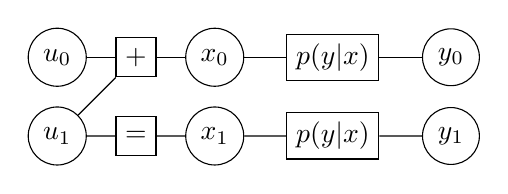
\begin{tikzpicture}[yscale=0.4, xscale=1, node distance=0.3cm, auto]
	
		\def \nodesize {0.5} %in cm
		\def \VertDist {2.5}
		\def \HorDist {1}
		\def \HorDisplace {0.5}
		
		\node (U0) at (0-\HorDist,0) [draw, circle, minimum width = \nodesize cm]{$u_0$};
		\node (U1) at (0-\HorDist,0-\VertDist) [draw, circle, minimum width = \nodesize cm]{$u_1$};%[align=center]{$U_1$};
		\node (Cn0) at (0,0) [draw, rectangle, minimum width = \nodesize cm,minimum height = \nodesize cm]{$+$};
		\node (Cn1) at (0,0-\VertDist) [draw, rectangle, minimum width = \nodesize cm,minimum height = \nodesize cm]{$=$};	
		\node (X0) at (\HorDist,0) [draw, circle, minimum width = \nodesize cm]{$x_0$};
		\node (X1) at (\HorDist,0-\VertDist) [draw, circle, minimum width = \nodesize cm]{$x_1$};
		\node (Cn2) at (2*\HorDist +\HorDisplace,0) [draw, rectangle, minimum width = \nodesize cm,minimum height = \nodesize cm]{$p(y|x)$};
		\node (Cn3) at (2*\HorDist +\HorDisplace,0-\VertDist) [draw, rectangle, minimum width = \nodesize cm,minimum height = \nodesize cm]{$p(y|x)$};	
		\node (Y0) at (3*\HorDist +2*\HorDisplace,0) [draw, circle, minimum width = \nodesize cm]{$y_0$};
		\node (Y1) at (3*\HorDist +2*\HorDisplace,0-\VertDist) [draw, circle, minimum width = \nodesize cm]{$y_1$};
		
		
		%[draw,circle,cross,minimum width=0.5 cm]
		\draw[-] (U0) -- (Cn0);
		\draw[-] (U1) -- (Cn1);
		\draw[-] (Cn0) -- (X0);
		\draw[-] (Cn1) -- (X1);
		\draw[-] (U1) -- (Cn0);
		\draw[-] (X0) -- (Cn2) --(Y0);
		\draw[-] (X1) -- (Cn3) --(Y1);
		
%		\node[draw,dashed,fit=(U0) (X1)] {};
		%\node[draw,dotted,color = darkred, fit=(U0) (X1),line width=1.0pt,line cap=round, dash pattern=on 0pt off 2\pgflinewidth] (block) {};
	
	\end{tikzpicture}